Il data science si riduce all'applicazione di metodi statistici, questi
metodi servono a collezionare dati, analizzarli e descriverli.

Sarà possibile fare inferenze, cioè cercare di trarre delle conclusioni
su una popolazione avendo un campione significativo.

\section{Data types}\label{data-types}

Le variabili possono essere:

\begin{itemize}
\item
  Categoriche, rappresentano un gruppo di oggetti, risposte si/no,
  divise a loro volta in:

  \begin{itemize}
  \item
    Nominali, i gruppi non possono essere messi in una scala.
  \item
    Ordinali, i gruppi possono essere messi in una scala.
  \end{itemize}
\item
  Numeriche, divise in:

  \begin{itemize}
  \item
    Discrete
  \item
    Continue
  \end{itemize}
\end{itemize}

\section{Experimental probability}\label{experimental-probability}

\begin{itemize}
\item
  \textbf{Trial}: osservazione di un evento e registro il risultato.
\item
  \textbf{Esperimento}: un insieme di trial.
\item
  \textbf{Sample space}: tutti i possibili risultati che posso ottenere.
\item
  \textbf{Probabilità}: rapporto tra l'evento che mi interessa e tutti i
  risultati possibili.
\item
  \textbf{Valore atteso}: valore medio che mi aspetto quando ripeto
  l\textquotesingle esperimento molte volte. Si ottiene sommando i
  prodotti fra probabilità di un certo valore per il valore stesso.
\end{itemize}

\begin{quote}
Per esempio avendo due dadi da 6 facce il valore medio che uscirà sarà 7
perchè è quello con più combinazioni possibili.

\textbf{SALTIAMO DA SLIDE 10 A 15}
\end{quote}

\section{Distribuzione di
probabilità}\label{distribuzione-di-probabilituxe0}

Descrive tutti i valori assunti dalla variabile e ad ciascun valore
associa il conteggio o la probabilità. La distribuzione viene descritta
tramite:

\begin{itemize}
\item
  \textbf{media {[}μ{]}:} \emph{somma di tutti i valori / numero di
  valori},
\item
  \textbf{varianza:} misura di quanto la distribuzione è
  ``appiattita''/allargata. \emph{La somma di tutte le distanze fra
  individuo e media, ciascuna al quadrato / numero di individui},
\item
  \textbf{deviazione standard {[}α{]}}: radice quadrata della varianza,
\end{itemize}

\subsubsection{Misure di tendenza
centrale}\label{misure-di-tendenza-centrale}

Ecco alcune misure di tendenza centrale:

\begin{itemize}
\item
  \textbf{media}: come prima,
\item
  \textbf{mediana}: numero nel mezzo di un dataset ordinato,
\item
  \textbf{moda}: valore più frequente.
\end{itemize}

\subsubsection{Misure di asimmetria}\label{misure-di-asimmetria}

Qui la misura principale è la \textbf{skewness}, cioè se i dati sono
concentrati da un lato preciso.

Se \emph{media \textgreater{} mediana} abbiamo una skew \emph{positiva}
quindi i \emph{dati si concentrano verso il lato SX} con coda a DX
(valori estremi che spostano la media). Invece è \emph{negativa} se
\emph{media \textless{} mediana} e si ha una \emph{coda verso SX}.

\subsubsection{Misure di variabilità}\label{misure-di-variabilituxe0}

Ci sono la varianza e la deviazione standard.

\subsubsection{Misura di correlazione}\label{misura-di-correlazione}

Misura di quanto due variabili siano correlate tra loro, sia ha:

\begin{itemize}
\item
  \textbf{Covarianza}
\item
  \textbf{Correlazione lineare}: esiste il metodo su pandas, valore
  compreso fra -1 e 1, più è vicino a 1 più c'è correlazione (si
  seguono), più è vicino a -1 c'è correlazione opposta (prendono `strade
  diverse') e con 0 non c'è tipo di correlazione.
\end{itemize}

\begin{quote}
In un scatter plot sono rappresentate in questo modo:
\end{quote}

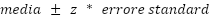
\includegraphics[width=6.26772in,height=1.51389in]{media/image1.png}

\subsubsection{Distribuzioni discrete e
continue}\label{distribuzioni-discrete-e-continue}

Nelle discrete ogni risultato univoco è assegnata una probabilità, nelle
continue ogni valore può assumere tutti i valori in un certo intervallo,
quindi non possiamo associare ad ogni valore preciso una percentuale ma
la assoceremo ad un range di valori.

Alcuni esempi di discreta sono:

\begin{itemize}
\item
  \textbf{Distribuzione uniforme}: ogni variabile ha la stessa
  probabilità di assumere qualsiasi valore all\textquotesingle interno
  di un intervallo specificato, es: lancio di un dado, ogni faccia ha la
  stessa \% di uscita.
\item
  \textbf{Distribuzione binomiale:} distribuzione del possibile numero
  di esiti positivi in un dato numero di prove in ciascuna delle quali
  esiste la stessa probabilità di successo.
\end{itemize}

Alcuni esempi di continue:

\begin{itemize}
\item
  \textbf{Normal distribution}: o gaussiana, è simmetrico rispetto alla
  media, mostrando che i dati vicini alla media sono più frequenti
  rispetto ai dati lontani dalla media. Sostanzialmente ha la seguente
  proprietà: se partendo dalla media tolgo o aumento una deviazione
  standard avrò un intervallo dove si avrà il 68,3 \% della popolazione,
  se mi sposto di due deviazioni avrò il 95.4\% della popolazione.
\end{itemize}

\begin{quote}
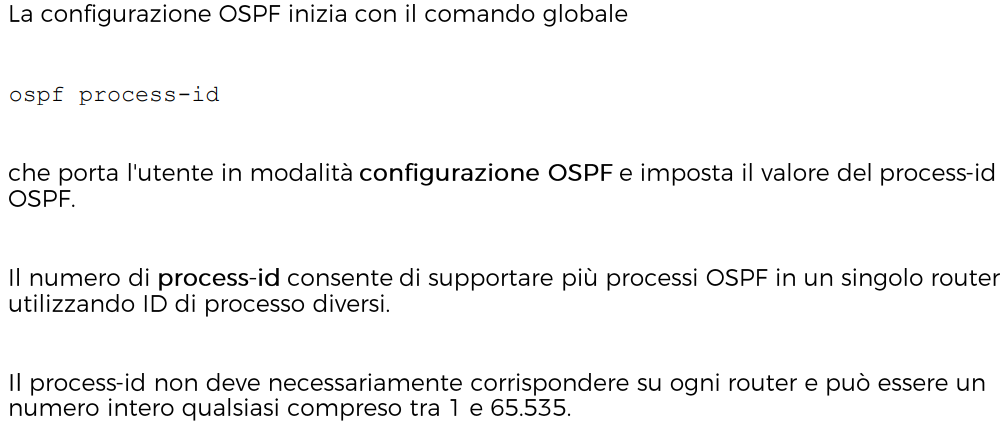
\includegraphics[width=4.47489in,height=2.98078in]{media/image4.png}

Di sotto c'è la tabella che rappresenta di quanto dobbiamo aggiungere o
togliere per avere la percentuale di popolazione:
\end{quote}

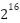
\includegraphics[width=4.59896in,height=4.3163in]{media/image3.png}

\section{Popolazione e campione}\label{popolazione-e-campione}

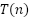
\includegraphics[width=6.26772in,height=4.01389in]{media/image5.png}

\section{Teorema del limite centrale}\label{teorema-del-limite-centrale}

Prendendo un insieme di campioni random da una popolazione più grande e
facendo la media otterremo un valore che va bene anche per l'intera
popolazione, questo è vero grazie a questo teorema.

\emph{Prendendo più campioni e facendo sempre le medie e mettendole
tutte in un grafico queste si distribuiranno tramite una
gaussiana/distribuzione normale e non importa com'era la distribuzione
di partenza.}

\section{Errore standard}\label{errore-standard}

Se nel teorema precedente prendiamo campioni sempre più piccoli la media
risultante sarà affetta da un errore sempre più grande, al contrario più
il campione è grande più l'errore diminuisce.

L'errore standard segue la formula:

\emph{deviazione standard / radice del numero di campioni}

\section{Intervalli e livelli di
confidenza}\label{intervalli-e-livelli-di-confidenza}

Come detto prima se dalla media ci spostiamo di + o - due (1.960 per
l\textquotesingle esattezza) valori dalla deviazione standard avremo il
95\% circa della popolazione, quindi abbiamo la sicurezza che ad ogni
calcolo al 95\% la media cada la dentro, ma è possibile che un campione
cadi fuori con una percentuale del 5\%

\emph{L'intervallo di confidenza è un range, che va dalla media -
l'errore alla media + l'errore, con la media nel mezzo,
all\textquotesingle interno del quale si stima che possa trovarsi il
vero valore di un parametro di interesse. Il livello invece è la
probabilità, che la media calcolata tramite campione ha, di cadere lì
dentro.}

Per trovare l'intervallo c'è la formula:

\(media\  \pm \ z\ *\ errore\ standard\)

dove la z la prendiamo dalla tabella in modo da ottenere la percentuale
voluta che il valore cada dentro l'intervallo.

Quindi usando la formula otteniamo due valori (uno calcolando con il +
l'altro con il -) che sono gli estremi dell'intervallo che ha la
percentuale, data da z, di quanto un valore possa cadere lì dentro.

\section{Test di ipotesi}\label{test-di-ipotesi}

Serve per verificare che un dato ottenuto da una popolazione sia
effettivamente significativo.

I passaggi sono:

\begin{itemize}
\item
  \textbf{imporre l'ipotesi nulla}: il caso base, se per esempio
  vogliamo valutare se i tiri con i dadi che abbiamo fatto siano veri
  l'ipotesi nulla è dire che il dado sia regolare e che quindi tutte le
  facce escano con la stessa frequenza;
\item
  \textbf{settare un livello di significabilità} \(\alpha\): per esempio
  voglio essere sicuro al 95\% quindi alfa sarà 95:
\item
  \textbf{calcolo la probabilità}: il p-value, cioè quanto è raro che il
  risultato ottenuto possa avvenire.
\end{itemize}

Per concludere se il p-value \textless{} \(\alpha\) allora posso
rifiutare/rigettare l'ipotesi nulla.

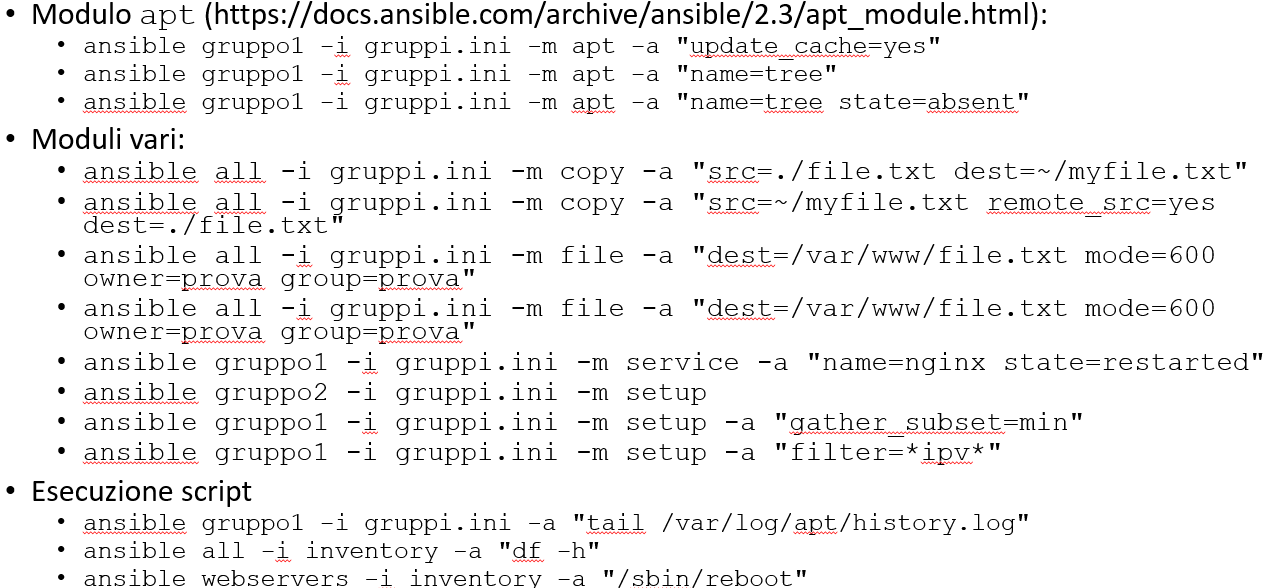
\includegraphics[width=3.88111in,height=2.32738in]{media/image2.png}

I test sono diversi e si differenziano in aspetti come il numero di
campioni, e sono:

\begin{itemize}
\item
  \textbf{T-test:} confrontare due gruppi/categorie di variabili
  numeriche con un campione di piccole dimensioni
\item
  \textbf{Z-test:} confrontare due gruppi/categorie di variabili
  numeriche con un campione di grandi dimensioni
\item
  \textbf{ANOVA test}: confrontare la differenza tra due o più
  gruppi/categorie di variabili numeriche
\item
  \textbf{Chi-Squared test}: esaminare la relazione tra due variabili
  categoriche
\item
  \textbf{Correlation test}: esaminare la relazione tra due variabili
  numeriche
\end{itemize}

Regressione lineare

Fa parte del machine learning supervisionato, quindi forniamo l'input e
label cioè la descrizione dell'input.

In questo caso abbiamo variabili indipendenti e fornisco l'output atteso
in modo da allenare il modello.

La regressione lineare è un modello che cerca di trovare la relazione
fra più variabili indipendenti e una variabile dipendente. Nel dettaglio
il modello va a trovare la retta che descrive meglio la relazione fra i
valori, quindi il coefficiente della retta che si avvicina di più ai
valori sullo scatter plot.

Quindi avremo una funzione:

\(y\  = \ b_{0} + b_{1} \cdot x\)

Dove:

\begin{itemize}
\item
  \textbf{y}: variabile dipendente
\item
  \textbf{x}: variabili indipendente
\item
  \(b_{0}\): intercetta, l'alzata all'origine cioè dove l'x è 0 l'y
  assume il valore di 0
\item
  \(b_{1}\): coefficiente angolare, la pendenza della retta e dice la
  variazione delle x al variare delle y.
\end{itemize}

Per individuare questa retta è definita una \textbf{Cost function}, che
dà la somma delle misure fra la distanza dei punti e la retta (fra y e
y) al quadrato diviso poi il numero di punti.

L'obiettivo del modello sarà poi quello di trovare i coefficienti in
modo che la cost function sia la più piccola possibile.

Esiste l'\textbf{R quadro} che serve per capire la bontà del modello,
per farlo calcoliamo la distanza fra i punti e la retta tracciata nel
punto medio di y, perché se i punti sono distanti tra loro senza
correlazione la retta creata dal modello non sarà mai buona come quella
della media; in sostanza:

Se la retta è buona \(R^{2}\) è uguale a 1

Time series

Nell\textquotesingle analizzare le serie storiche possiamo farlo in due
modi: con scomposizione o modellistica (usato da noi).

Una serie storica è stazionaria se non c'è correlazione con il tempo e
se oscilla tra un medesimo valore, inoltre non ci devono essere trend e
stagionalità.

Nella funzione di autocorrelazione globale, detta anche ACF, i picchi
determinano una correlazione fra ogni variabile della serie e k valori
indietro.

Per esempio un picco su 1 indica che c'è correlazione tra ogni valore
della serie e il valore precedente, se c'è sul 2 indica che c'è
correlazione tra ogni valore della serie e il valore che ricorre due
valori precedenti.
